\documentclass[a4paper]{article}

\usepackage{array}

\usepackage{hopsantut}

\begin{document}
\maketitle{Getting Started}

\section*{Program Overview}
Before you build your own first Hopsan model, it is necessary to understand the different parts of the graphical user interface. After starting Hopsan and opening a model, it will look like the picture bellow.  

\begin{figure}[ht]
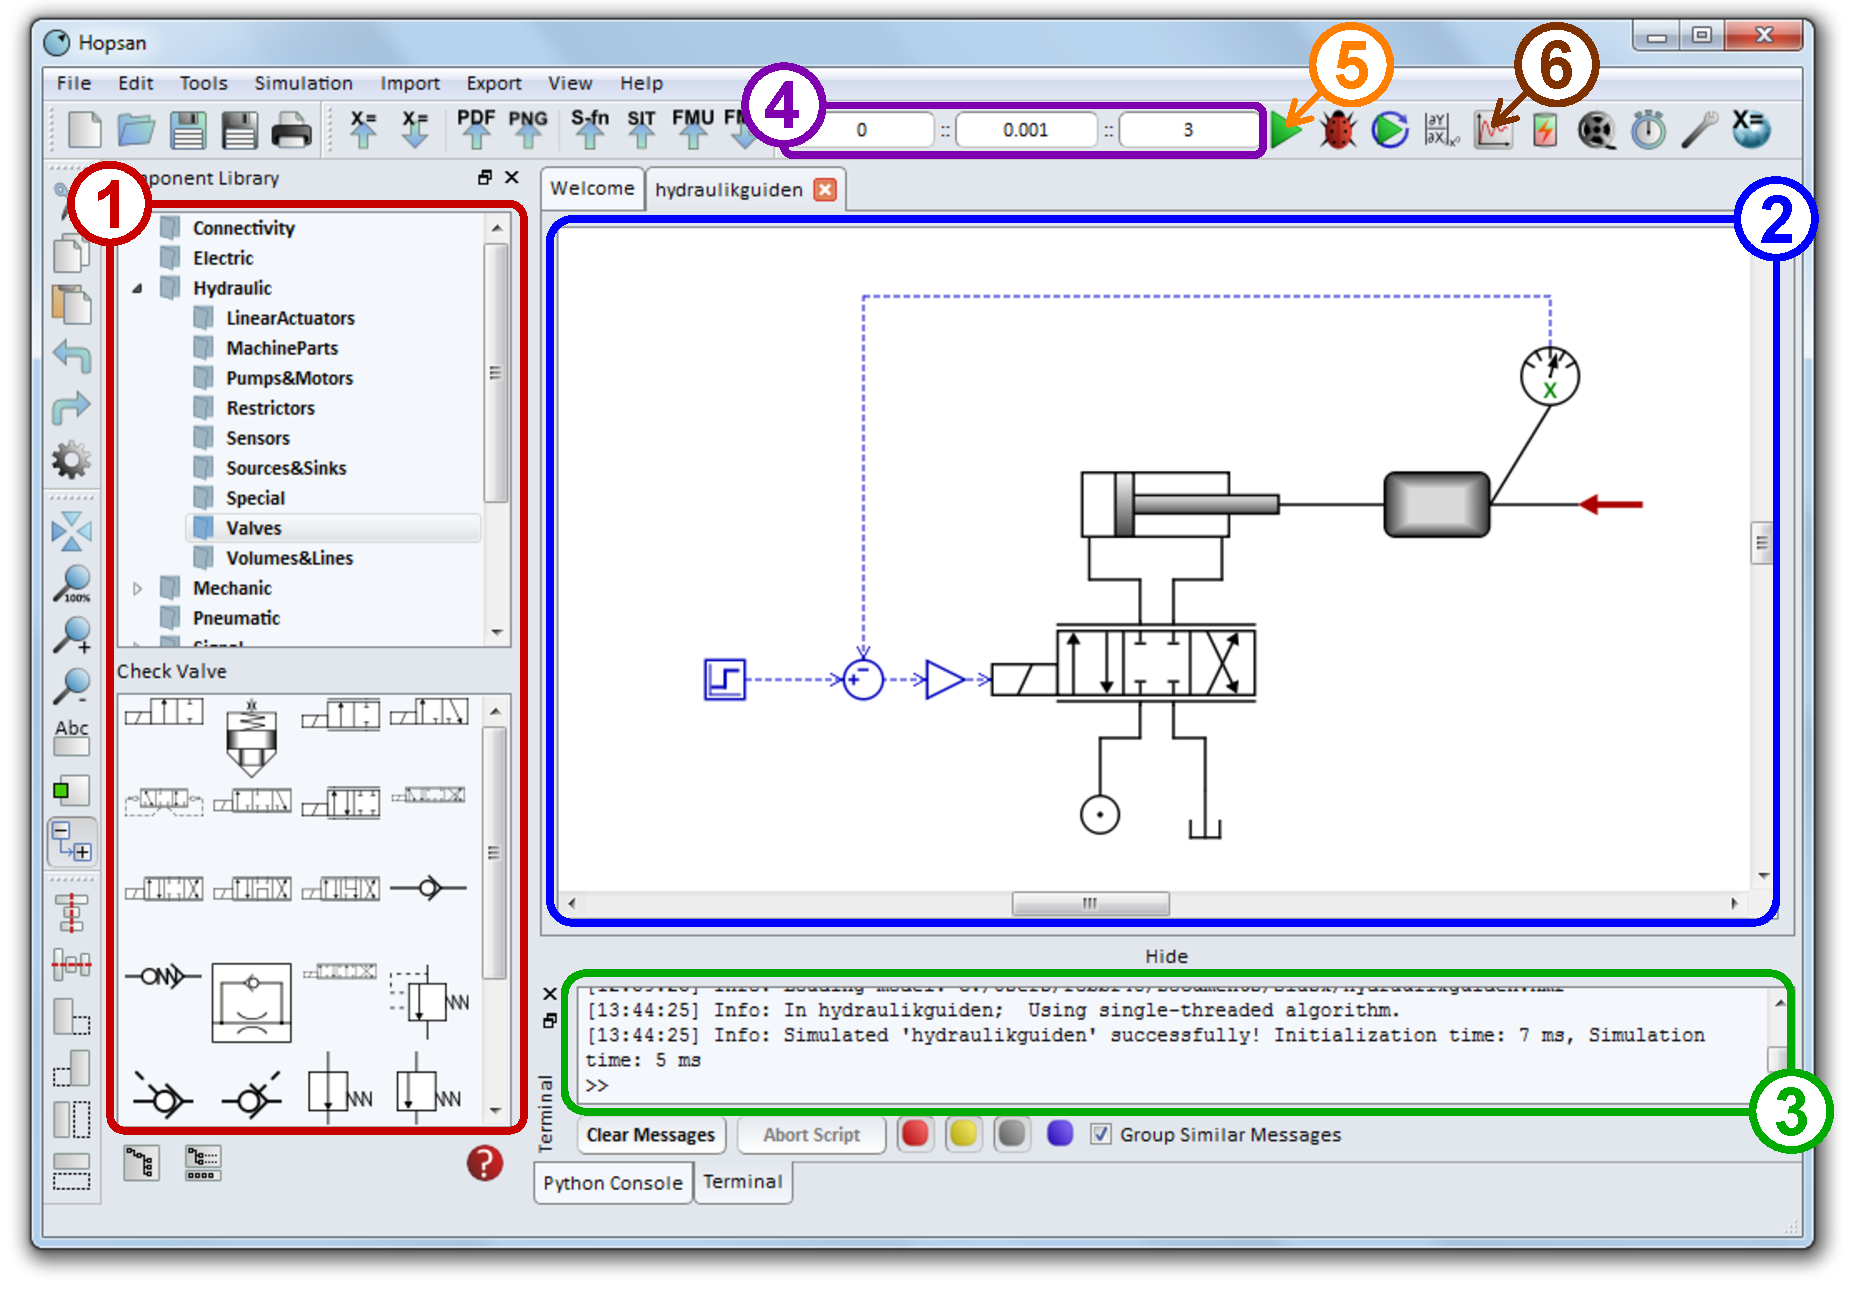
\includegraphics[width=\textwidth]{gfx/screenshot.pdf}
\end{figure}

\begin{enumerate}
\item \textbf{Component Library}\\
All loaded component libraries are shown here. Components are sorted in libraries based on their relative directories. To add a component to the model, simply drag it to the workspace and drop it.

\item \textbf{Workspace}\\
Models are shown in the main workspace. All added components are shown, and they can be connected as desired. Right-clicking on a component opens a menu with various alternatives. From here it is possible to open the Properties dialog, from where the components parameters can be modified. This can also be accessed directly by double-clicking the component. 

\item \textbf{Command terminal} \\
The terminal widget shows output messages from Hopsan. These are coloured depending on their type; black for information, orange for warnings, red for errors and blue for debugging. Be extra careful with the red messages, as these will often tell you that you have done something wrong. It is also possible to give commands to Hopsan from the terminal, or to call external script files in the HCOM language. This is, however, too advanced for this guide. Write ?help? for more detailed information. 

\item \textbf{Simulation time settings} \\
This is where the simulation start time, time step and stop time can be controlled. It is for example possible to start the simulation before t=0, to avoid logging initial transients for a model that does not start in steady-state. Reducing the time step will increase the accuracy of the simulation, at the cost of longer simulation time. Number of log samples can be changed from the model properties dialog, accessed by the wrench icon.

\item \textbf{Simulation button} \\
Click here to start a simulation. If something is incorrect in your model, for example if a connection is missing, an error message will be shown in the terminal.

\item \textbf{Plot button} \\
Click here to open a list with all logged variables from the simulation. These can be plotted by double-clicking them, or by dragging them to the workspace. A plot window will look like this.

\begin{figure}[ht]
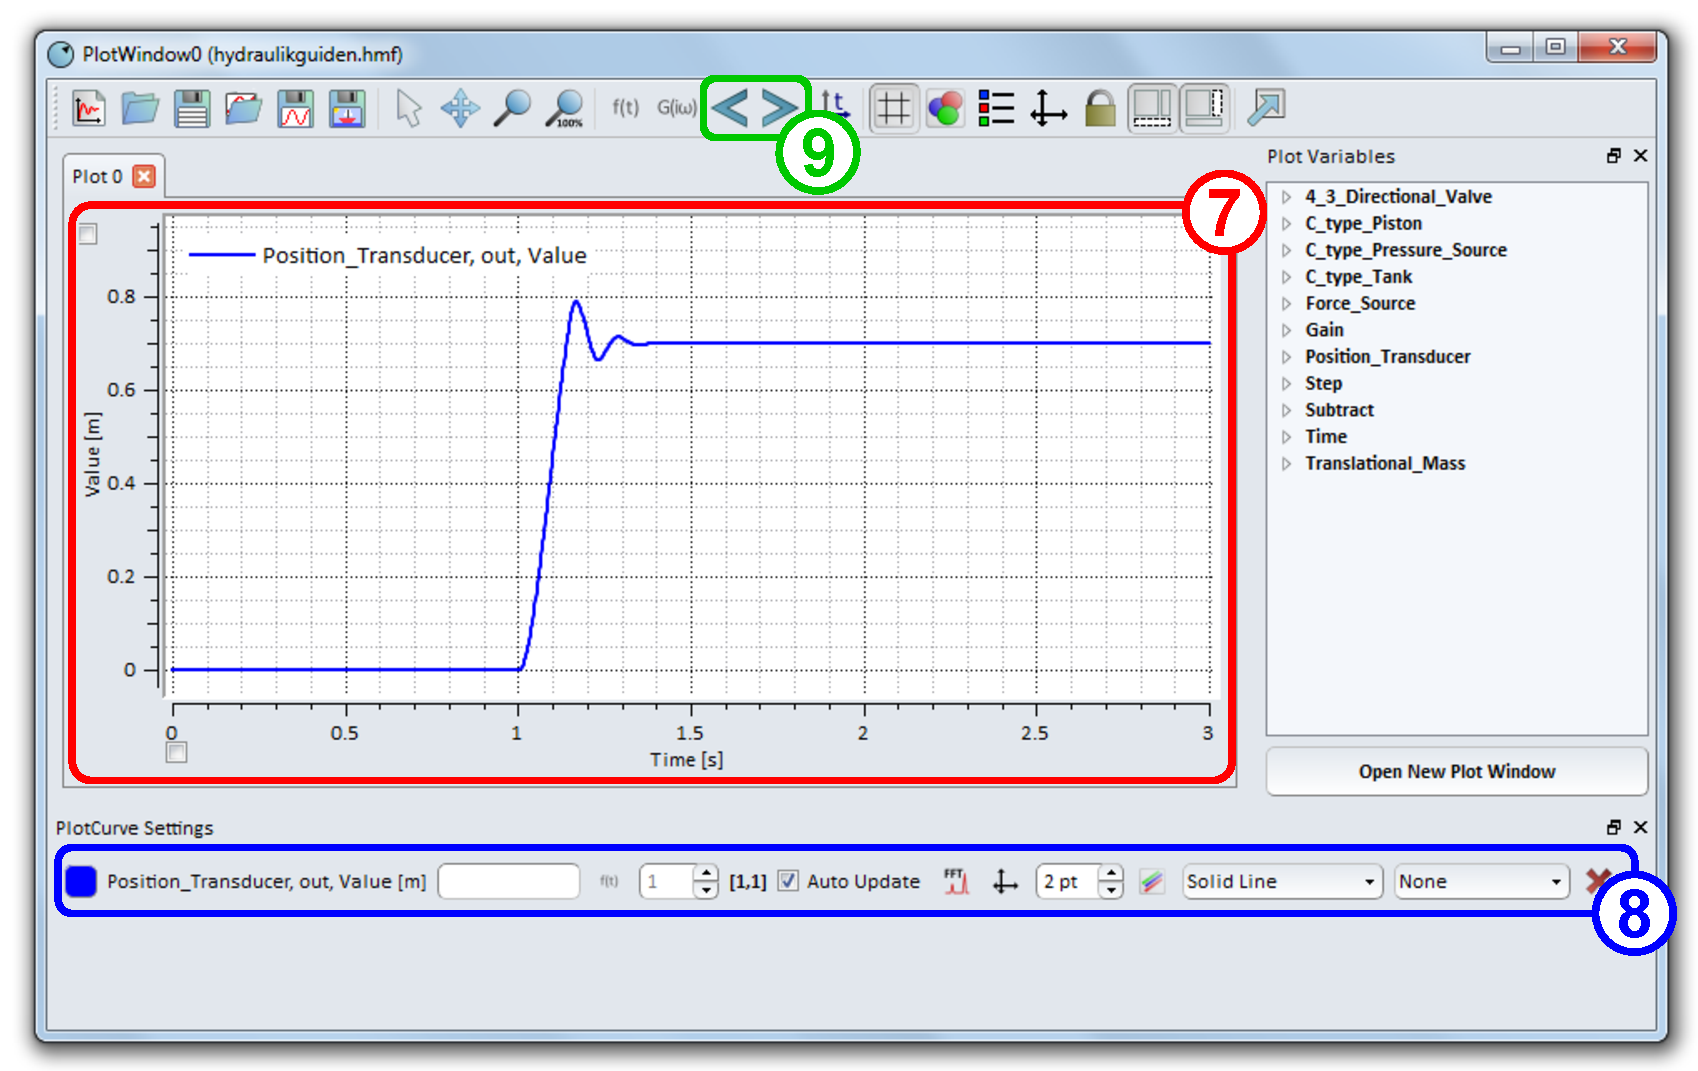
\includegraphics[width=\textwidth]{gfx/screenshot-plot.pdf}
\end{figure}

\item \textbf{Main plot area}
Plot curves are shown here. It is possible to add several curves to the same plot by dragging them to the left, right or bottom axes in the plot area. Right-click in the graph for more alternatives.

\item \textbf{Plot curve settings} \\
Appearance, generation, scaling and offset of a specific plot curve can be modified from here. It is also possible to remove the curve with the red X icon.

\item \textbf{Switch generation} \\
Log variables in Hopsan are grouped by generations. After every simulation a new generation with the logged results is created. These buttons makes it possible to increase or decrease the generation for all variables in a graph. Generations for individual curves are controlled in their plot curve settings as described in point 8. This makes it possible to compare different generation of a specific variable.
 
\end{enumerate}

\section*{Building a model}
This tutorial will show how to build the model shown in the figure above. The model consists of a hydraulic position servo, where a directional valve is used to control a piston connected to a translational inertia. A simple feedback loop is used to position the piston.
\begin{enumerate}
\item \textbf{Create a new model} \\
Click on New Model on the welcome screen, or on the icon in the toolbar:
 	
\icon{0}{gfx/Hopsan-New.png}{Create a new empty model}
 	
\item \textbf{Add components to the model} \\
The following components are required for the model. A component can be found by writing its name in the Filter box, or by finding it in the library hierarchy.

\vspace{5pt}
\foldericon{0}{Hydraulic}
\foldericon{1}{Valves}
\component{2}{4/3 Directional Valve}
\foldericon{1}{Sources \& Sinks}
\component{2}{C-type Pressure Source}
\component{2}{C-type Tank}
\foldericon{1}{Linear Actuators}
\component{2}{C-type Piston}
\foldericon{0}{Mechanic}
\foldericon{1}{Linear}
\component{2}{Translational Mass}
\component{2}{Force Source}
\component{2}{Position Transducer}
\foldericon{0}{Signal}
\foldericon{1}{Source \& Sinks}
\component{2}{Step}
\foldericon{1}{Arithmetics}
\component{2}{Subtract}
\component{2}{Gain}
\vspace{5pt}

\item \textbf{Connect the components} \\
The following components are required for the model. A component can be found by writing its name in the Filter box, or by finding it in the library hierarchy.

\icon{0}{gfx/Hopsan-ShowPorts.png}{Show unconnected ports (Ctrl-T)}

Hydraulic and mechanical ports are shown as green and red squares. Red arrows represent input and output signal ports. Hydraulic and mechanical ports also contain the letter C or Q. This tells the type of the component and is a result of the use of the transmission line element method (TLM). C-ports can only be connected to Q-ports and vice versa. Try making an erroneous connection on purpose, and not the resulting error message. Then connect all components according to figure 2.

\pagebreak
\item \textbf{Change parameter values} \\
In order to recreate the result shown in the graph above it is necessary to adjust som parameter values in the model. This is done from the Properties dialog, which can be accessed by double-clicking a component. The following parameters need to be changed:

{\renewcommand{\arraystretch}{1.2} 
\begin{tabularx}{\linewidth}{X X X}
\textbf{Component} & \textbf{Parameter} & \textbf{Value} \\
\specialrule{1.3pt}{0pt}{0pt}
C-type Pressure Source & $\mathit{p}$ & 2e7 \\
Step & $\mathit{y_{A}}$ & 0.7 \\
Gain & $\mathit{k}$ & 0.015
\end{tabularx}
}

\item \textbf{Simulate} \\
Set simulation start time, time step and stop time to 0, 0.001 and 3, respectively. Then press the simulate icon.

\icon{0}{gfx/Hopsan-Simulate.png}{Simulate current project (Ctrl-Shift-S)}

If everything is correct the simulation will now be executed. See the output in the terminal for more information.

\item \textbf{Plot the results} \\
Now plot the resulting value from the position transducer, by right-clicking on the Out-port and selecting ?Plot Value [m]?. You can also use the list of log variables as described in the previous section.

\icon{0}{gfx/Hopsan-Plot.png}{Plot variables (Ctrl-Shift-P)}

Log variables can also be exported to various formats and used in other programs. It is also possible to export the graph as a picture.

\item \textbf{Change a parameter and compare the results} \\
Now change the parameter k in the component Gain to 0.03, i.e. twice as high as before. Simulate again and go back to the plot window and change generation to compare the curves. It is also possible to add the same curve twice and see the two generations in the same graph.

\item \textbf{Animation} \\
Sometimes it is difficult to understand a system by just looking at the graphs. In the toolbar at the top there is a button that starts the animation function. Try clicking at it!

\icon{0}{gfx/Hopsan-Animation.png}{Animate}

This opens the animation mode. There is a new special toolbar that controls the animation. Click at the \textit{Play} icon to start an animation of the system you just simulated. 

\icon{0}{gfx/Hopsan-Play.png}{Start replay animation}

Return to the model by clicking the red X icon.
\end{enumerate}




\end{document}